\subsection{Modules} \label{subsec:modules}
\begin{figure}[!ht]
    \centering
    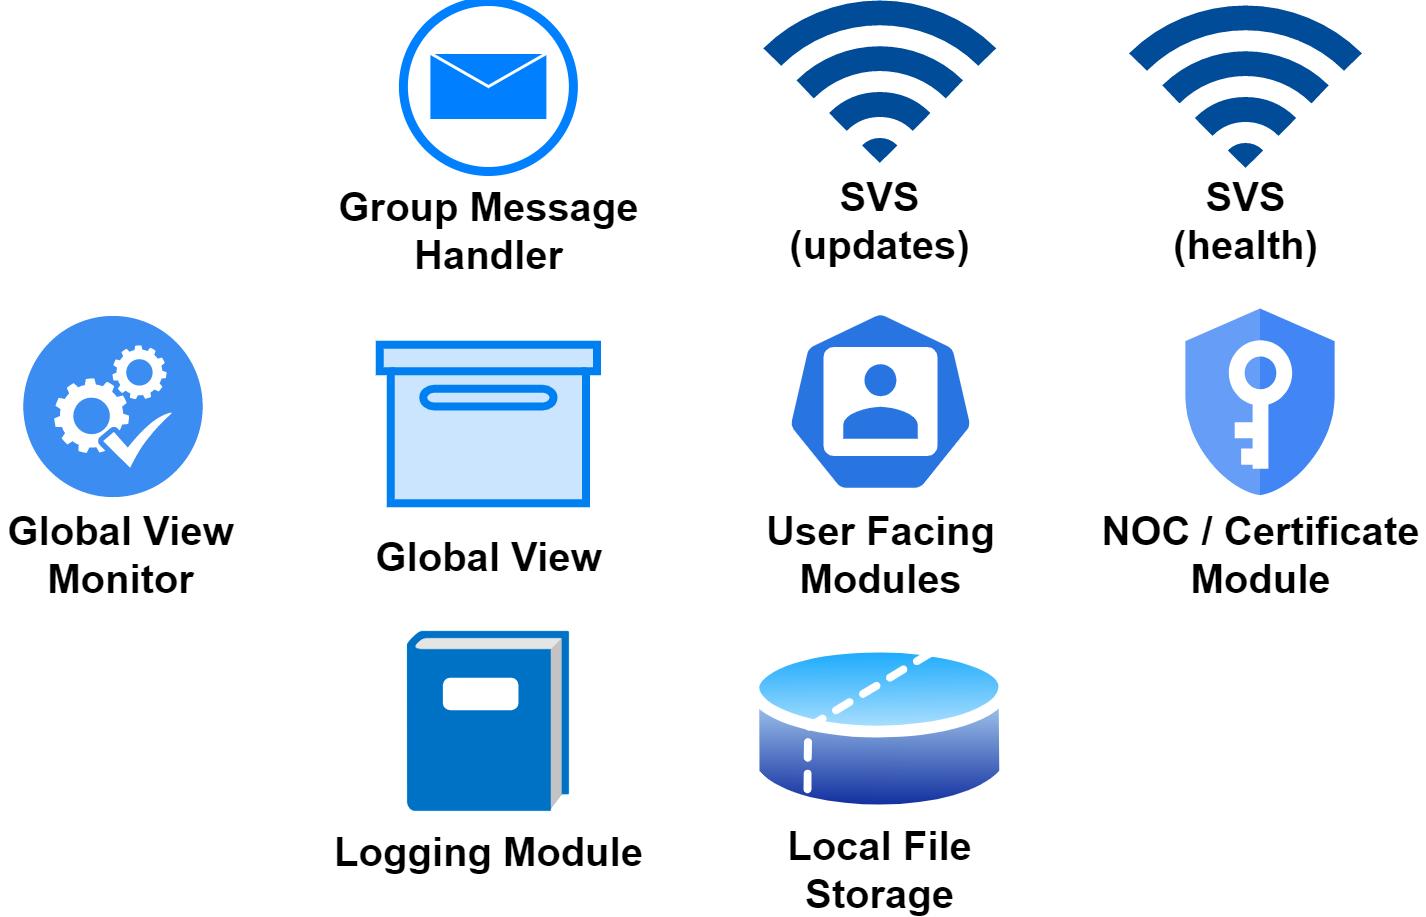
\includegraphics[width=\columnwidth]{visuals/node-modules.png}
    \caption{Modules that make up a Hydra Node}
    \label{fig:node-modules}
\end{figure}
%\todo[inline]{Lixia says - heartbeat tracker should be part of the global view monitor}

To provide the functions described in Subsection~\ref{subsec:functions}, a Hydra node is made up of several modules as illustrated in  Figure~\ref{fig:node-modules}. Nine modules make up a Hydra node, and the following list briefly describes each of them. 
%More information will be later explained further in the paper.

%\subsubsection{Heartbeat Tracker}
%The heartbeat tracker is a module in a Hydra node that a node uses to track all other nodes in the system. Each node sends a heartbeat every 30 seconds that is propagated using group messaging (SVS - see Module below) to all the other nodes. If a node X does not hear a heartbeat message from another node Y, it presumes node Y is unreachable and sets the node in the heartbeat tracker to ``Unreachable". 
%If a node comes back online after failure, it sends out a heartbeat message and node X sets node Y to be ``Alive"  in the heartbeat tracker.
%Heartbeat Tracker interacts with Global view, and Group message handler. 

%of all nodes within Hydra and periodically send out a heartbeat of its own.

\subsubsection{StateVectorSync (SVS)}
%The SVS protocol is used for the exchange of group messages between all nodes within Hydra (group messages - see Section 4.1). SVS will update node states, notifying other nodes of recent changes via Group Messages(GMs), which helps maintain a consistent view across nodes.  As mentioned above, SVS interacts with group messages.

The SVS module uses the SVS protocol to publish data (e.g., state update messages) that is received by all other nodes within Hydra. SVS allows Hydra to maintain a consistent view across the nodes.

\subsubsection{Global View}
%The global view contains complete information about the Hydra system, including all node information, all files and, for each \emph{file}, which nodes own and take over the file, as well as meta-info such as size, origin node, numbers of copy, etc (global view - see Section 4.4). Global View Monitor is only used to monitor the global view. Without the global view monitor, no node would do anything that supports other nodes. The monitor constantly checks the global view (which is constantly updated) and finds out what it needs to do, for example if it needs to fetch/store files.
The Global View is a local database to a Hydra node. It represents a node's view of the Hydra federation. The global view contains information related to the Hydra system such as files' metadata, node information, and replication information.

It also contains the heartbeat tracker sub-module that is used to send and track a heartbeat message. The heartbeat message establishes whether a node is alive or unavailable.  If the nodes in the federation do not hear a heartbeat message from a node for a certain time, it presumes the node is unreachable and sets the node in the heartbeat tracker to ``Unreachable". Once $n$ heartbeats are missed from a specific node, the nodes initiate automatic replication.



%and all files' metadata.


\subsubsection{Group Message Handler}
%All processes join a ``group" via SVS and synchronize the global view by publishing group messages. Group messages posted by a node are visible to all nodes, just like chatting in a group. Naturally, Group Message Handler interacts with SVS and Group messages.(group messages handler - see Section XX)

All Hydra nodes join a ``group" via SVS and synchronize the global view by publishing group messages. Group messages posted by a node are visible to all nodes. This module handles Group Messages - messages that are sent to the group of Hydra nodes. The group message handler interacts with SVS to receive and apply the new updates to Global view and publish new group messages.
%them and appropriately affecting the Hydra node based on them.


\subsubsection{Global View Monitor}
%This module constantly checks the global view (which is constantly updated) and finds out what the Hydra node needs to fetch or store.
The global view monitor monitors the global view database for any changes. If a change is detected, it initiates an outgoing update message. It also applies update messages received by the node to the Global view database.

\subsubsection{User-Facing Modules}
%The features within the hydra system that are available to users, including insert, delete, query, and retrieval. 
%When a node receives an Insertion command for a file, the node first correctly authenticates the command and then immediately starts fetching the file. When the file is stored, the node forms an "insert" GM and applies this GM to its global view (insertion - see Section 5.1).
%When a node receives a Deletion command, if the node has the file or a copy of this file, it deletes the file or the copy. The GM "delete" is generated by deleting the file to update its global view.(deletion - see Section 5.4).
%When a node receives a Query command, the node simply checks the query type information in the global view and returns it via packet. (querying - see Section 5.4).
%When a node receives a Retrieval command, there are 3 possible scenarios. (1) Hydra does not have the file; (2) The node does not have the file, but another node does; (3) The node has the file (retrieval - see Section 5.3).

These public-facing modules allow users to interact with the Hydra system, providing data insertion, deletion, and retrieval functionality. They also allow the user/applications to query the system for file availability. 

\subsubsection{Network Operation Center (NOC)}
%Acts as the system trust anchor for Hydra deployments, and issues the certificate. A new Hydra node fetches a trust anchor by sending an Interest and verifies the returned self-signed certificate out-of-band. Then the node signs the Interest and requests a certificate from the NOC. Finally, NOC signs the certificate using the trust anchor and returns it in the replied data. 
NOC is a centralized entity that acts at the root of trust for a deployment. NOC provides signed certificates to the nodes and users. %and key information in order be apart of the system.

\subsubsection{Logging Module}
%Enable logging globally for the entire hydra system to monitor and troubleshoot errors for easy optimization.

This module logs all node records (data operations and errors) to monitor Hydra and provide information to the administrator.

\subsubsection{Local File Storage}
%It's the module that writes files to the actual file system, garbage collects, and interfaces with Insertion/Deletion/Querying/Replication/Retrieval modules. It is also closely related to the storage size.
Local file storage is the Database on a node that holds the Data packets corresponding to a published file. The file storage module also performs garbage collection and deletes any file not accessed for a certain duration.
%This database stores the files that the Hydra node said it would store.